% ============================================
% CAPÍTULO 3 - PARTE II: ANÁLISE E TRANSMISSÃO DE SINAIS
% Seções 3.6 a 3.9
% ============================================

% ============================================
% SEÇÃO 3.6: EQUALIZAÇÃO (removida — conteúdo extra)
% ============================================
% \section{Equalização e Exemplos Práticos de Canais}
% \input{sec3_6_signal_distortion}

% ============================================
% SEÇÃO 3.7: ENERGIA E DENSIDADE ESPECTRAL DE ENERGIA
% ============================================
\section{Energia de Sinal e Densidade Espectral de Energia}
\input{sec3_7_energy_spectral_density}

% ============================================
% SEÇÃO 3.8: POTÊNCIA E DENSIDADE ESPECTRAL DE POTÊNCIA
% ============================================
\section{Potência de Sinal e Densidade Espectral de Potência}
\input{sec3_8_power_spectral_density}

% ============================================
% SEÇÃO 3.9: SINAIS DE BANDA BÁSICA E BANDA PASSANTE
% ============================================
\section{Sinais de Banda Básica e Banda Passante}
% ============================================
% SEÇÃO: SINAIS DE BANDA BÁSICA E BANDA PASSANTE
% Desenvolvimento passo a passo: passante → analítico → banda básica → I/Q
% ============================================

\subsection{Sinais de Banda Básica e Banda Passante}

\begin{frame}{O que é um Sinal de Banda Básica?}

Um sinal de \textbf{banda básica} (baseband) tem energia concentrada em torno de $f = 0$:

\[
X(f) \approx 0 \quad \text{para} \quad |f| > W
\]

onde $W$ é a \textbf{largura de banda} do sinal.

\vspace{0.2cm}

\textbf{Exemplos:}
\begin{itemize}
\item Voz humana: $W \approx 4$ kHz
\item Sinal de áudio: $W \approx 20$ kHz
\item Dados digitais a 1 Mbps: $W \approx 500$ kHz
\item Sinal de vídeo: $W \approx 6$ MHz
\end{itemize}

\textbf{Característica principal:} O espectro está centrado na origem ($f = 0$).

\end{frame}

% ============================================

\begin{frame}{O que é um Sinal de Banda Passante?}

Um sinal de \textbf{banda passante} (passband) tem energia concentrada em torno de uma frequência portadora $f_c \gg W$:

\[
S(f) \approx 0 \quad \text{para} \quad |f - f_c| > W \; \text{e} \; |f + f_c| > W
\]

\textbf{Exemplos:}
\begin{itemize}
\item Rádio AM: $f_c \approx 1$ MHz, $W = 5$ kHz
\item Rádio FM: $f_c \approx 100$ MHz, $W = 200$ kHz
\item Wi-Fi: $f_c = 2.4$ GHz, $W = 20$ MHz
\item 5G: $f_c = 3.5$ GHz, $W = 100$ MHz
\end{itemize}

\textbf{Característica principal:} O espectro está centrado em $\pm f_c$.

\end{frame}

% ============================================

\begin{frame}{Banda Básica vs Banda Passante — Visualização}

\begin{center}
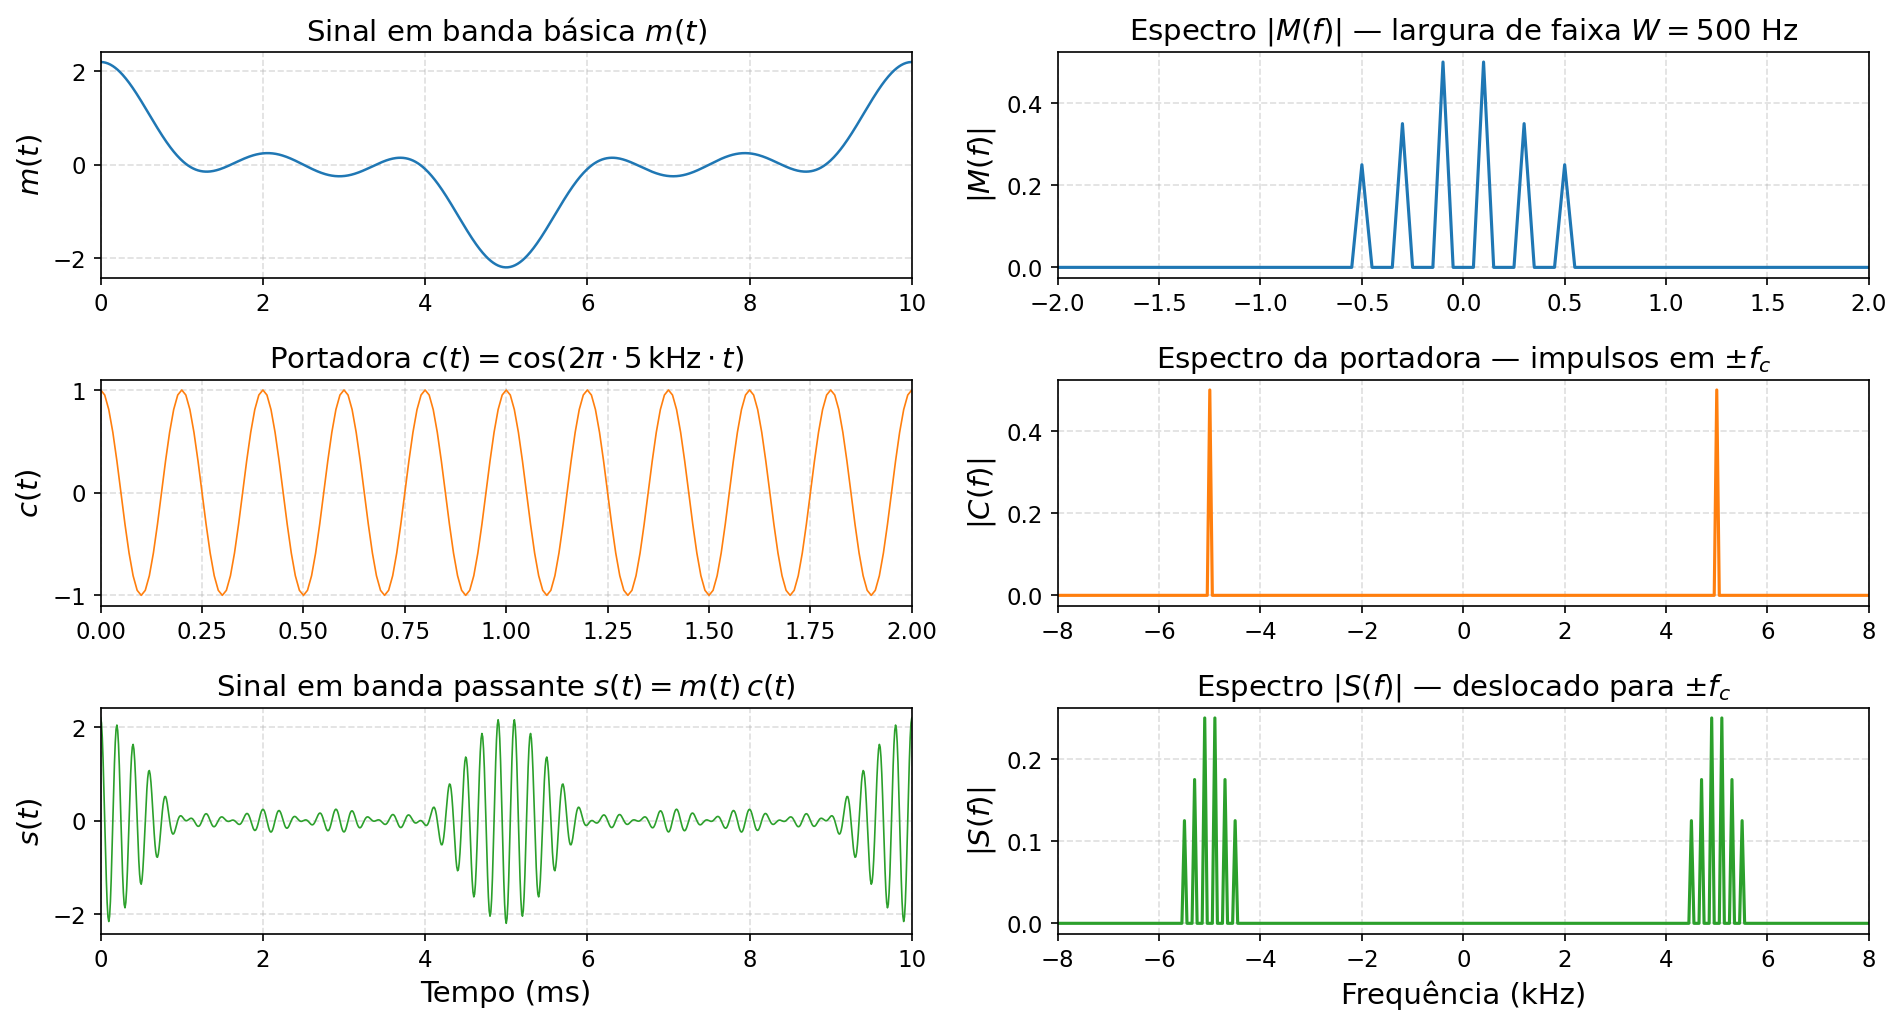
\includegraphics[width=\figFull, height=0.85\textheight, keepaspectratio]{figures/cap3/banda_basica_vs_passante}
\end{center}

\end{frame}

% ============================================

\subsection{Do Sinal Passante à Representação em Banda Básica}

\begin{frame}{Passo 1: Espectro do Sinal Passante}

Considere um sinal passante real $s(t)$ centrado em $f_c$.

Como $s(t)$ é \textbf{real}, seu espectro é simétrico: $S(-f) = S^*(f)$.

\begin{center}
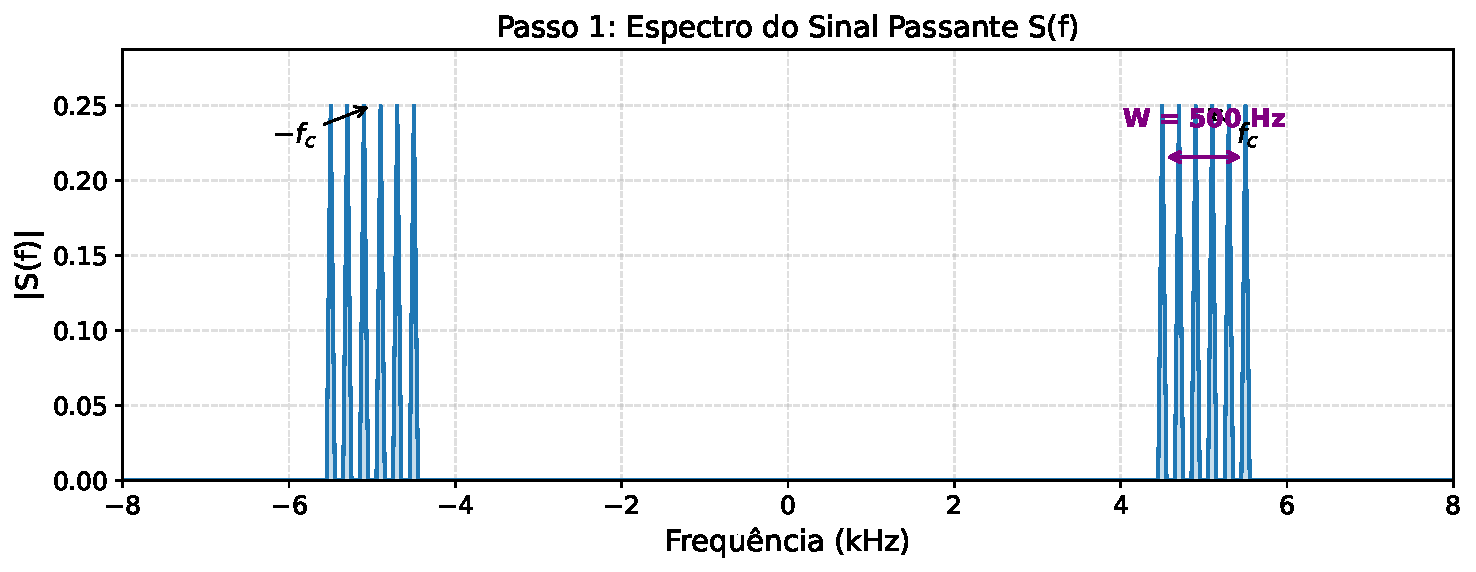
\includegraphics[width=\figFull, height=0.60\textheight, keepaspectratio]{figures/cap3/passband_passo1_espectro}
\end{center}

A informação em $f < 0$ é \textbf{redundante} — vem da simetria Hermitiana.

%\textbf{Pergunta:} Podemos trabalhar apenas com as frequências positivas?

\end{frame}

% ============================================

\begin{frame}{Passo 2: Manter Apenas Frequências Positivas}

Multiplicamos $S(f)$ por $2u(f)$ (degrau unitário na frequência):

\[
Z(f) = 2\,S(f) \cdot u(f) = \begin{cases} 2S(f), & f > 0 \\ 0, & f < 0 \end{cases}
\]

\begin{center}
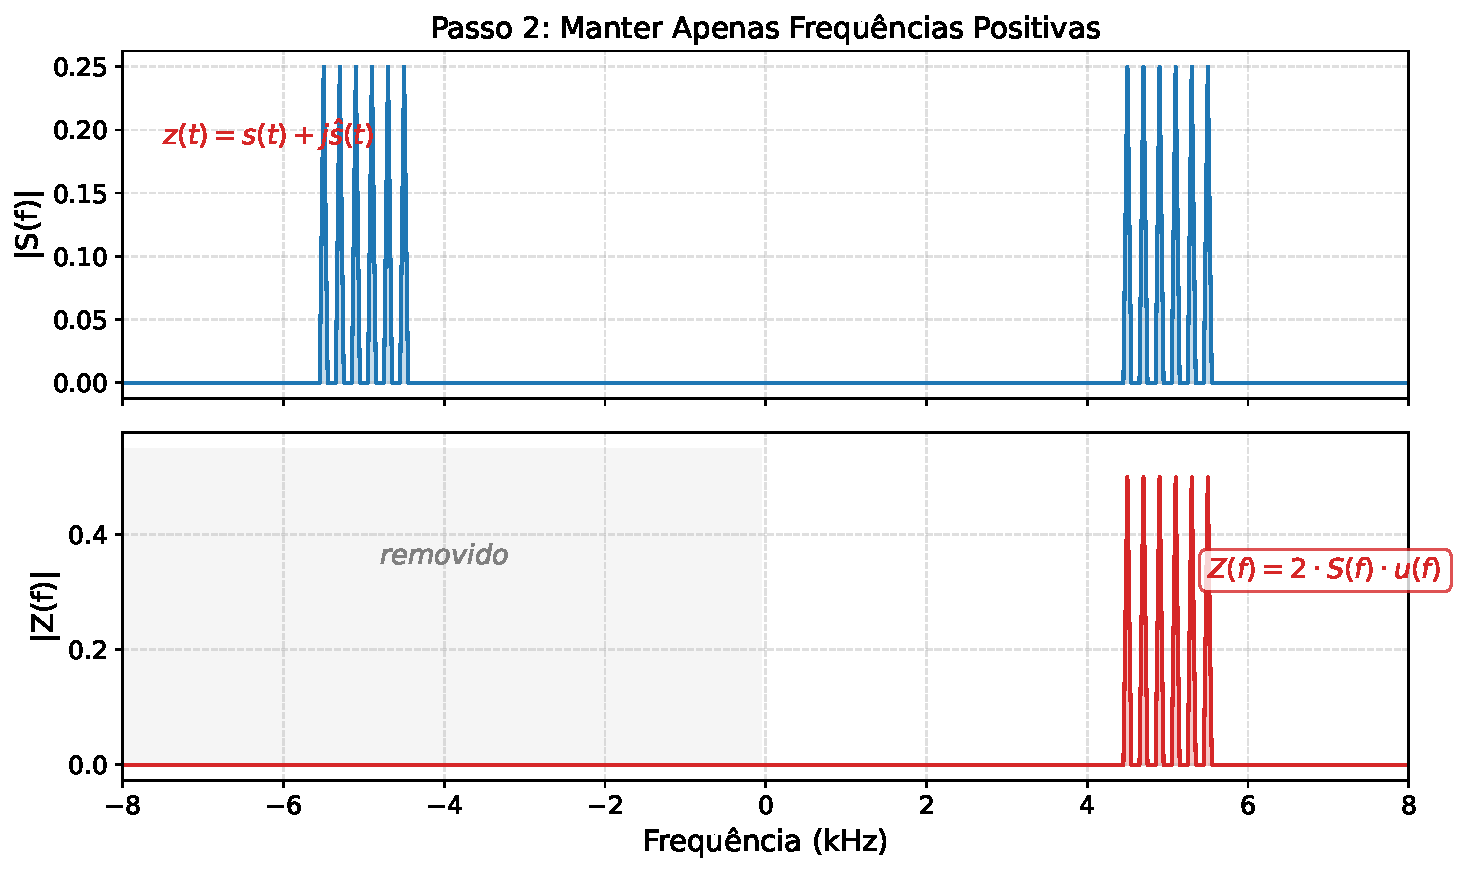
\includegraphics[width=\figFull, height=0.55\textheight, keepaspectratio]{figures/cap3/passband_passo2_analitico}
\end{center}

\end{frame}

% ============================================

\begin{frame}{Passo 2: Sinal Analítico}

O sinal $z(t)$ correspondente é chamado \textbf{sinal analítico} de $s(t)$.

\end{frame}

% ============================================

\begin{frame}{Passo 3: Deslocar para Banda Básica}

Deslocamos $Z(f)$ de $-f_c$: \quad $\tilde{S}(f) = Z(f + f_c)$ \quad No tempo: $\tilde{s}(t) = z(t) \cdot e^{-j2\pi f_c t}$

\begin{center}
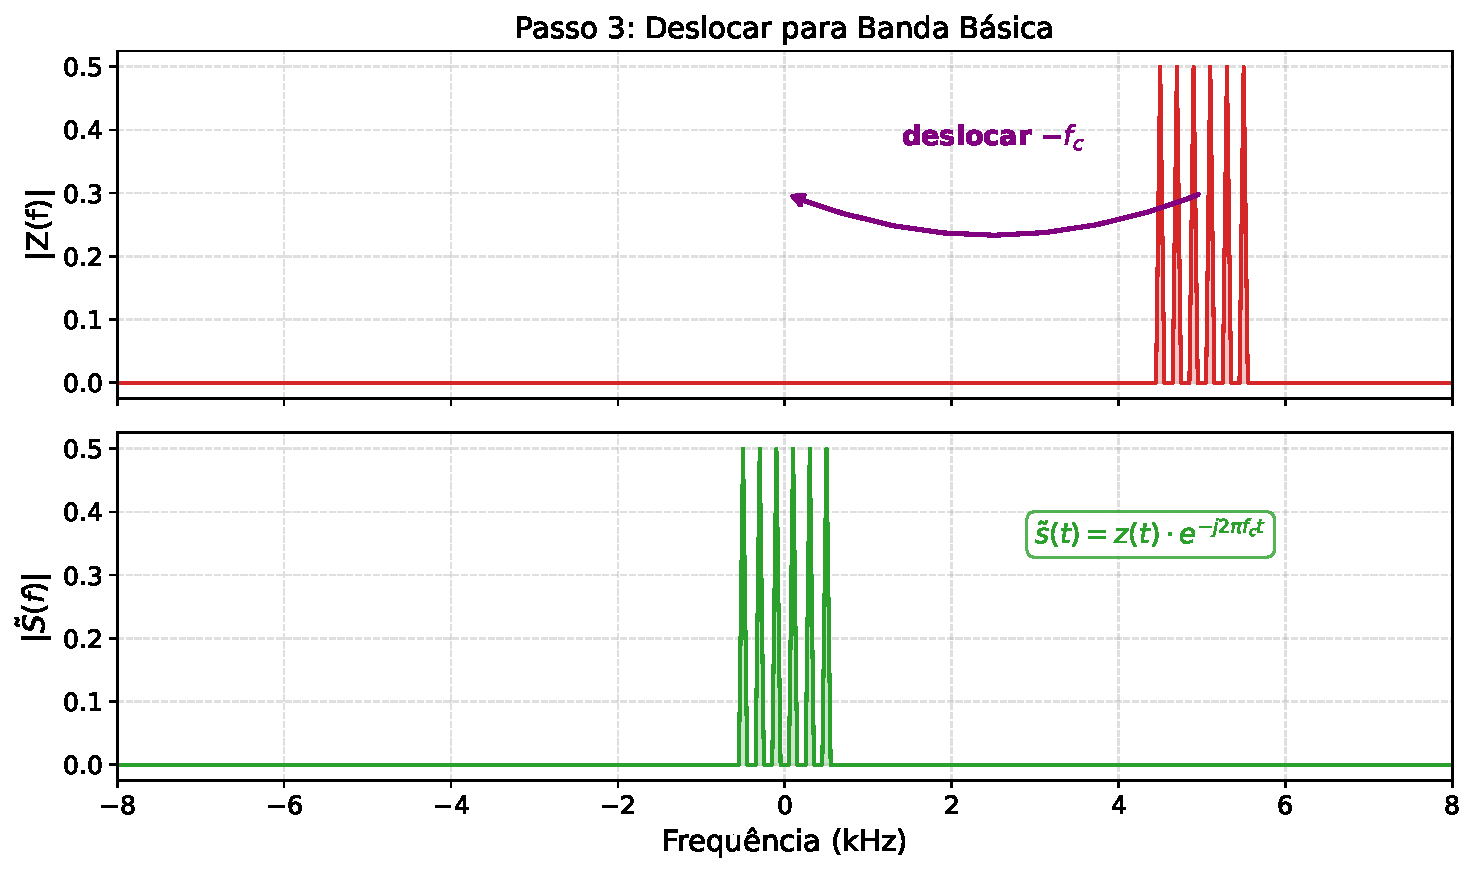
\includegraphics[width=\figFull, height=0.65\textheight, keepaspectratio]{figures/cap3/passband_passo3_desloc}
\end{center}

$\tilde{s}(t)$ é o \textbf{envelope complexo} — sinal de banda básica com toda a informação do sinal passante.

\end{frame}

% ============================================

\subsection{A Transformada de Hilbert}

\begin{frame}{De Onde Vem a Transformada de Hilbert? (1/2)}

No Passo 2, multiplicamos por $2u(f) = 1 + \sgn(f)$:

\begin{center}
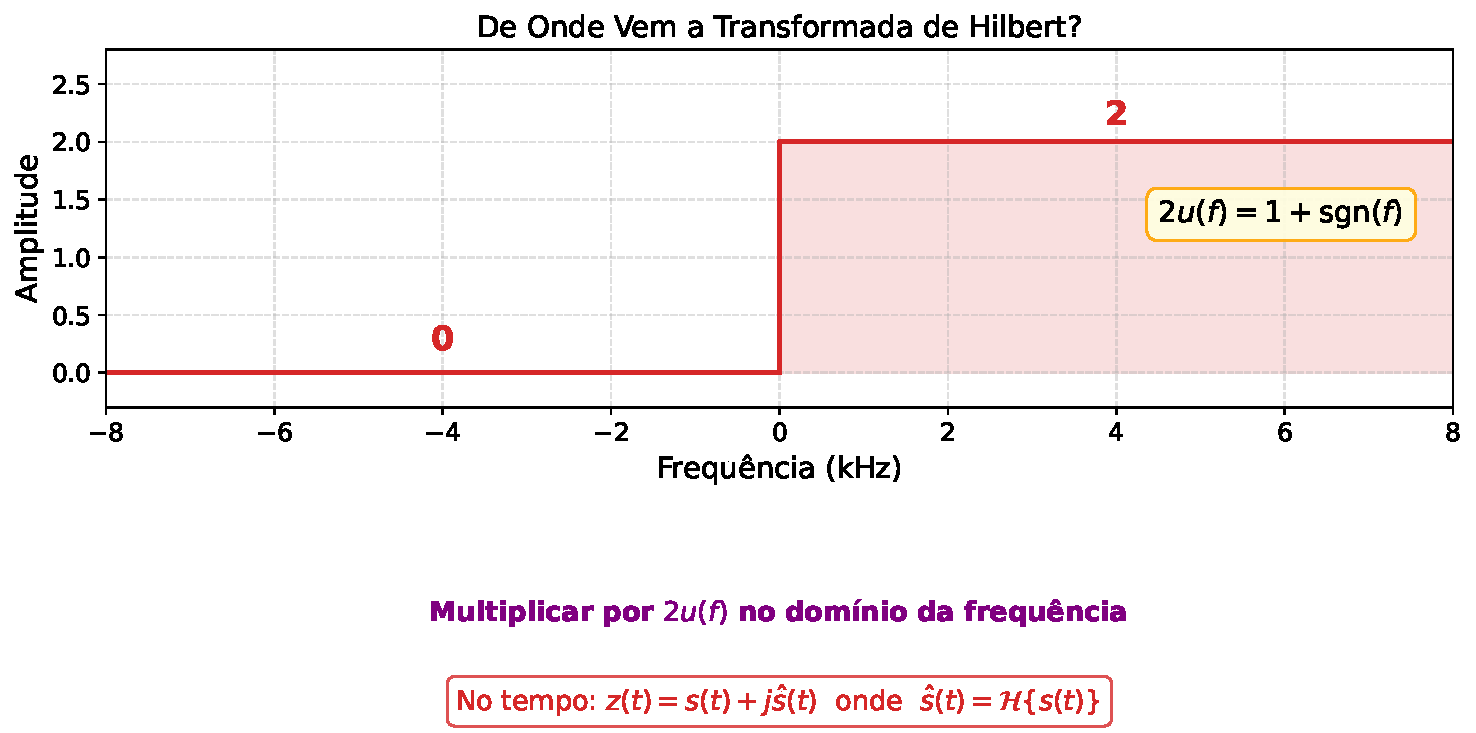
\includegraphics[width=\figHalf, height=0.3\textheight, keepaspectratio]{figures/cap3/passband_passo4_hilbert}
\end{center}
\vspace{-2mm}

No domínio da frequência:
\[
Z(f) = S(f)\big[1 + \sgn(f)\big] = S(f) + \sgn(f) \cdot S(f)
\]

Sabemos que multiplicação na frequência $\Leftrightarrow$ convolução no tempo:
\[
z(t) = \mathcal{F}^{-1}\{S(f)\} + \mathcal{F}^{-1}\{\sgn(f) \cdot S(f)\}
\]

O primeiro termo é simplesmente $s(t)$. Mas o que é $\mathcal{F}^{-1}\{\sgn(f) \cdot S(f)\}$?

\end{frame}

% ============================================

\begin{frame}{De Onde Vem a Transformada de Hilbert? (2/2)}

Sabemos que $\dfrac{1}{\pi t} \leftrightarrow -j\,\sgn(f)$, logo $\sgn(f) \leftrightarrow \dfrac{j}{\pi t}$.

Pelo teorema da convolução:
\[
\mathcal{F}^{-1}\{\sgn(f) \cdot S(f)\} = s(t) \ast \frac{j}{\pi t} = j\underbrace{\left[s(t) \ast \frac{1}{\pi t}\right]}_{\hat{s}(t)}
\]

\textbf{Definimos} a Transformada de Hilbert: \quad $\hat{s}(t) \triangleq s(t) \ast \dfrac{1}{\pi t}$

Portanto: \quad $\mathcal{F}^{-1}\{\sgn(f) \cdot S(f)\} = j\,\hat{s}(t)$

\vspace{3mm}
Substituindo na expressão de $z(t)$:
\[
\boxed{z(t) = s(t) + j\,\hat{s}(t)}
\]

onde $\hat{s}(t)$ é a \textbf{Transformada de Hilbert} de $s(t)$: defasagem de $90°$ em cada componente.

\end{frame}

% ============================================

\begin{frame}{Propriedades da Transformada de Hilbert}

\textbf{No domínio da frequência:}
\[
\hat{S}(f) = -j \cdot \sgn(f) \cdot S(f)
\]

\textbf{Efeito:}
\begin{itemize}
\item Para $f > 0$: multiplica por $-j$ $\Rightarrow$ \textbf{atrasa $90°$}
\item Para $f < 0$: multiplica por $+j$ $\Rightarrow$ \textbf{adianta $90°$}
\item \textbf{Não altera a magnitude}: $|\hat{S}(f)| = |S(f)|$
\end{itemize}

\textbf{Exemplos:} $\cos(2\pi f_0 t) \xrightarrow{\mathcal{H}} \sin(2\pi f_0 t)$, \quad $\sin(2\pi f_0 t) \xrightarrow{\mathcal{H}} -\cos(2\pi f_0 t)$

\end{frame}

% ============================================

\begin{frame}{Transformada de Hilbert — Visualização}

\begin{center}
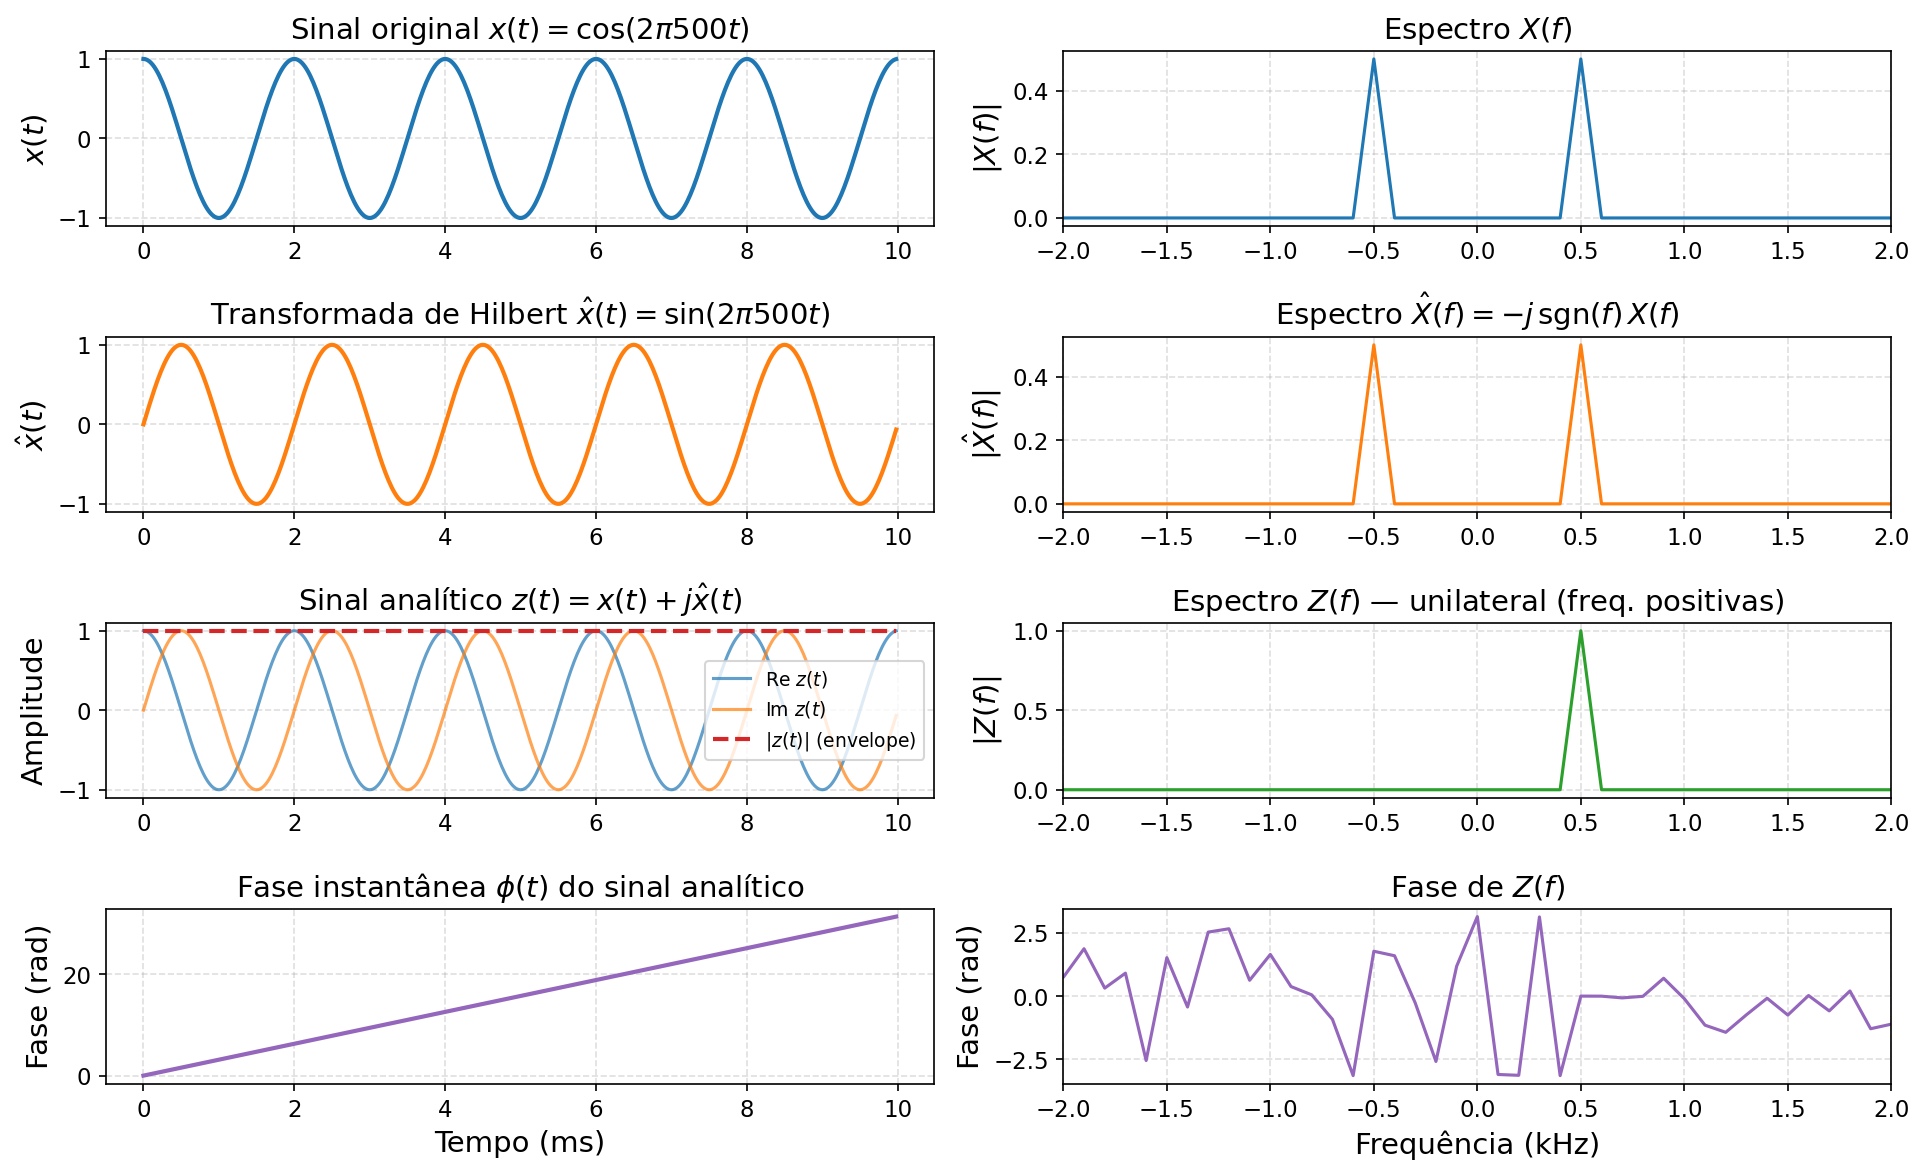
\includegraphics[width=\figFull, height=0.85\textheight, keepaspectratio]{figures/cap3/hilbert_transform}
\end{center}

\end{frame}

% ============================================

\subsection{Componentes em Fase e Quadratura}

\begin{frame}{Componentes I e Q}

O envelope complexo $\tilde{s}(t)$ é um sinal complexo de banda básica.

Separamos em parte real e imaginária:

\[
\boxed{\tilde{s}(t) = s_I(t) + j\,s_Q(t)}
\]

\begin{itemize}
\item $s_I(t) = \Real\{\tilde{s}(t)\}$: componente \textbf{em fase} (In-phase)
\item $s_Q(t) = \Imag\{\tilde{s}(t)\}$: componente \textbf{em quadratura} (Quadrature)
\end{itemize}

\begin{center}
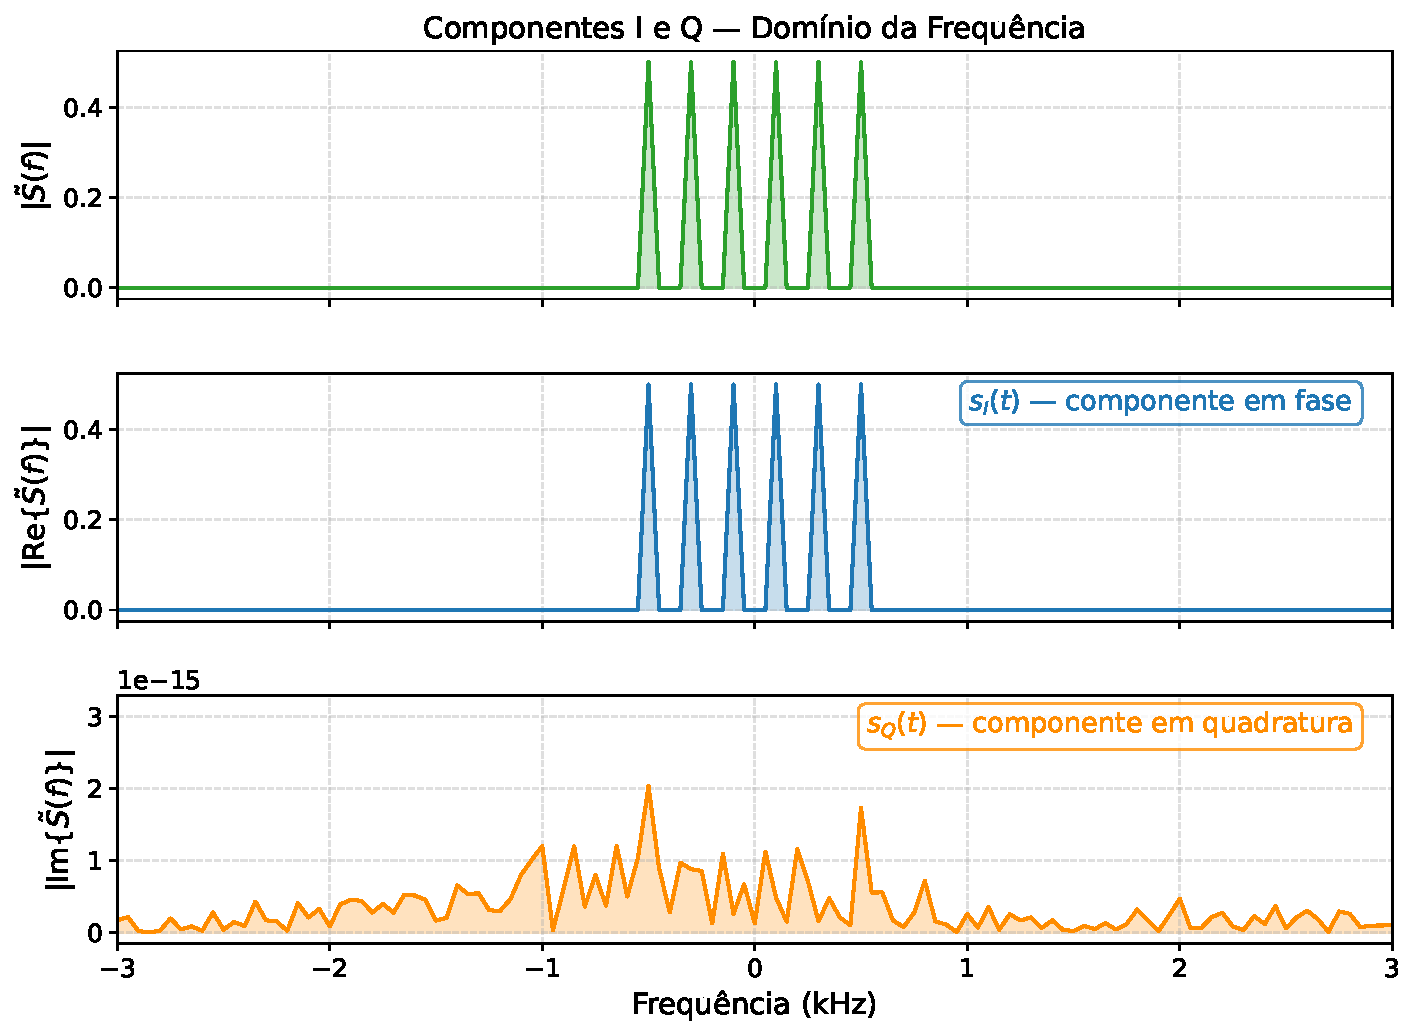
\includegraphics[width=\figHalf, height=0.45\textheight, keepaspectratio]{figures/cap3/passband_passo5_IQ}
\end{center}

\end{frame}

% ============================================

\begin{frame}{O Sinal de Banda Básica é Complexo — Representação Vetorial}

O envelope complexo $\tilde{s}(t) = s_I(t) + j\,s_Q(t)$ é um \textbf{sinal complexo}.

Em cada instante $t$, é um \textbf{vetor} no plano I/Q:

\begin{columns}[c]
\begin{column}{0.45\textwidth}
\begin{center}
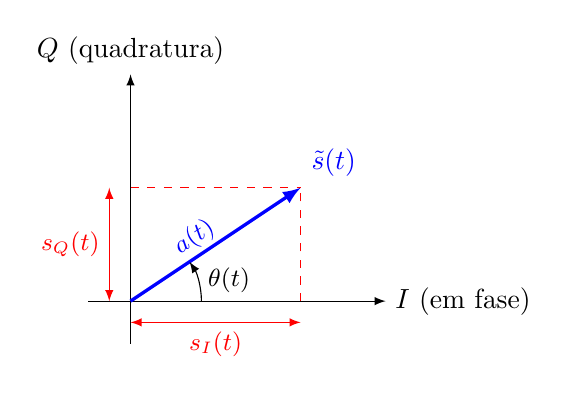
\begin{tikzpicture}[scale=1.8, >=latex]
% Axes
\draw[->] (-0.3,0) -- (1.8,0) node[right] {$I$ (em fase)};
\draw[->] (0,-0.3) -- (0,1.6) node[above] {$Q$ (quadratura)};
% Vector
\draw[->, very thick, blue] (0,0) -- (1.2,0.8) node[above right] {$\tilde{s}(t)$};
% Components
\draw[dashed, red] (1.2,0) -- (1.2,0.8);
\draw[dashed, red] (0,0.8) -- (1.2,0.8);
\draw[<->, red] (0,-0.15) -- node[below, font=\small] {$s_I(t)$} (1.2,-0.15);
\draw[<->, red] (-0.15,0) -- node[left, font=\small] {$s_Q(t)$} (-0.15,0.8);
% Angle
\draw[->] (0.5,0) arc (0:33.7:0.5) node[midway, right, font=\small] {$\theta(t)$};
% Magnitude
\node[blue, font=\small, rotate=33.7] at (0.45,0.45) {$a(t)$};
\end{tikzpicture}
\end{center}
\end{column}
\begin{column}{0.52\textwidth}
\textbf{Amplitude} (magnitude do vetor):
\[
a(t) = |\tilde{s}(t)| = \sqrt{s_I^2(t) + s_Q^2(t)}
\]

\textbf{Fase} (ângulo do vetor):
\[
\theta(t) = \arctan\!\left(\frac{s_Q(t)}{s_I(t)}\right)
\]
\end{column}
\end{columns}

\end{frame}

% ============================================

\begin{frame}{Representação Vetorial — Forma Polar}

\textbf{Forma polar} do envelope complexo:
\[
\boxed{\tilde{s}(t) = a(t)\,e^{j\theta(t)}}
\]

onde $a(t) = |\tilde{s}(t)|$ é a \textbf{amplitude instantânea} e $\theta(t) = \arctan\!\left(\frac{s_Q(t)}{s_I(t)}\right)$ é a \textbf{fase instantânea}.

\vspace{0.3cm}

Toda a informação do sinal passante (amplitude \textbf{e} fase) está codificada neste vetor complexo de banda básica.

\end{frame}

% ============================================

\begin{frame}{Reconstrução: Banda Básica $\to$ Banda Passante}

\begin{columns}[c]
\begin{column}{0.48\textwidth}
Para recuperar o sinal passante:

\[
\boxed{s(t) = \Real\left\{\tilde{s}(t) \cdot e^{j2\pi f_c t}\right\}}
\]

Expandindo:

\[
\boxed{s(t) = s_I\cos(2\pi f_c t) - s_Q\sin(2\pi f_c t)}
\]
\end{column}
\begin{column}{0.50\textwidth}
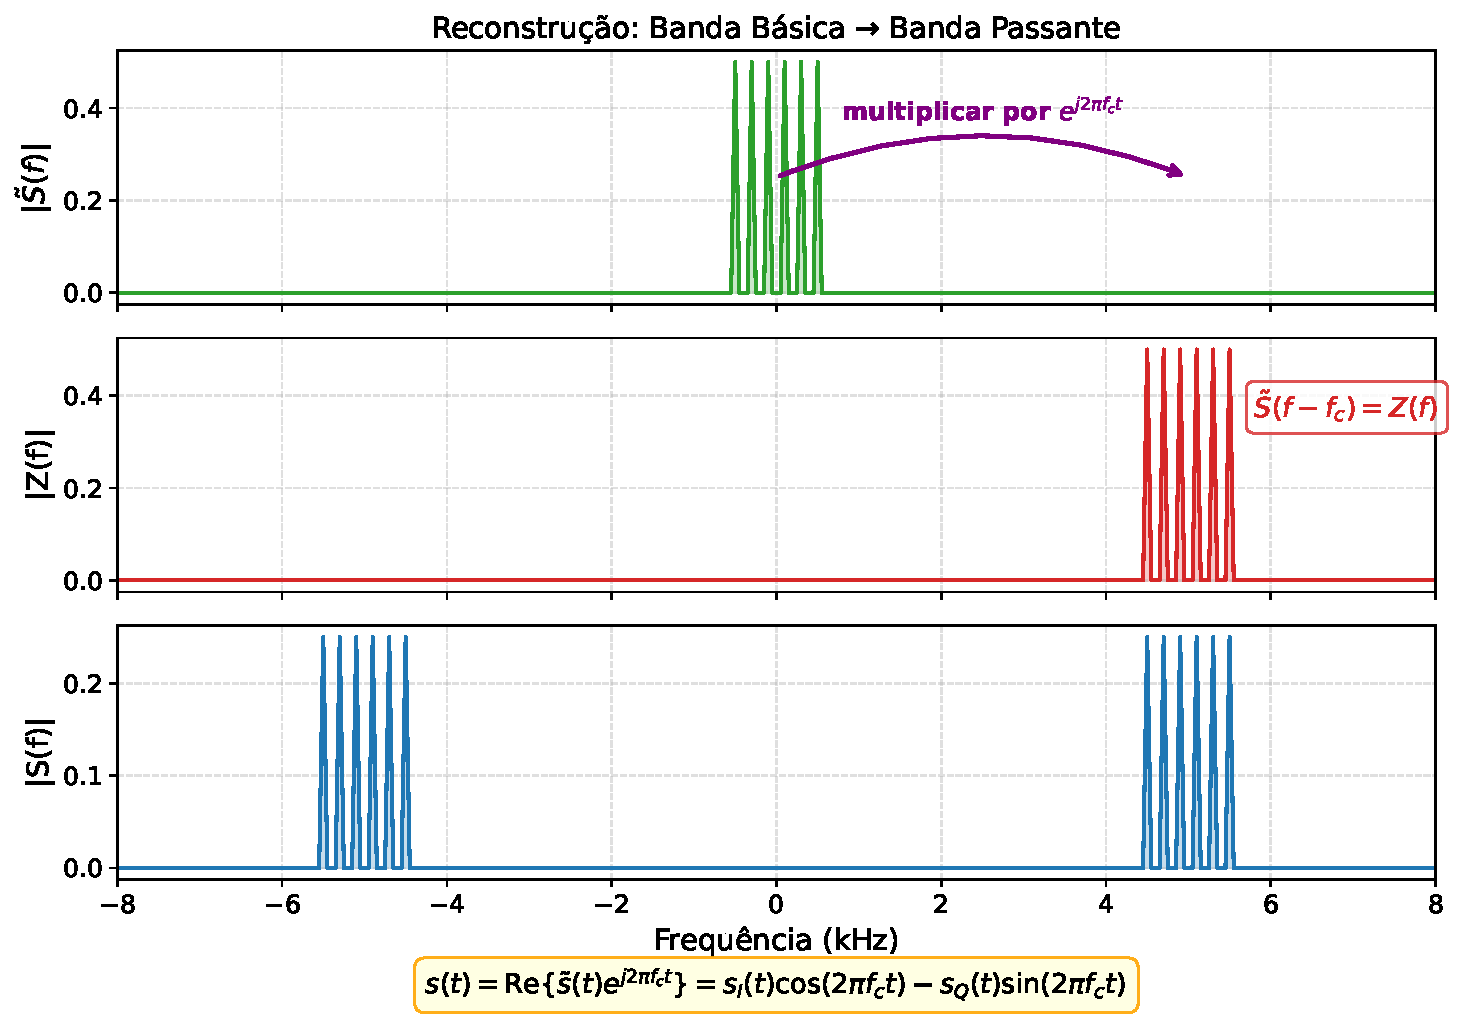
\includegraphics[width=\textwidth]{figures/cap3/passband_passo6_reconstrucao}
\end{column}
\end{columns}

\end{frame}

% ============================================

\begin{frame}{Obtendo $\hat{s}(t)$ a partir das Componentes I/Q}

Sabemos que o sinal analítico é $z(t) = s(t) + j\,\hat{s}(t)$.

Por outro lado, usando o envelope complexo:
\[
z(t) = \tilde{s}(t)\,e^{j2\pi f_c t} = \big[s_I(t) + j\,s_Q(t)\big]\big[\cos(2\pi f_c t) + j\sin(2\pi f_c t)\big]
\]

Expandindo e separando parte real e imaginária:

\begin{align*}
s(t) &= \Real\{z(t)\} = s_I(t)\cos(2\pi f_c t) - s_Q(t)\sin(2\pi f_c t) \\[6pt]
\hat{s}(t) &= \text{Im}\{z(t)\} = s_I(t)\sin(2\pi f_c t) + s_Q(t)\cos(2\pi f_c t)
\end{align*}

\end{frame}

% ============================================

\begin{frame}{Representação Matricial — Modulação I/Q}

Podemos escrever $s(t)$ e $\hat{s}(t)$ de forma compacta:

\[
\boxed{
\begin{bmatrix} s(t) \\ \hat{s}(t) \end{bmatrix}
=
\underbrace{
\begin{bmatrix}
\cos(2\pi f_c t) & -\sin(2\pi f_c t) \\
\sin(2\pi f_c t) & \cos(2\pi f_c t)
\end{bmatrix}
}_{\text{matriz de rotação por } 2\pi f_c t}
\begin{bmatrix} s_I(t) \\ s_Q(t) \end{bmatrix}
}
\]

\vspace{3mm}

A portadora aplica uma \textbf{rotação} ao vetor de banda básica $(s_I, s_Q)$:
\begin{itemize}
\item O vetor $(s_I, s_Q)$ gira com velocidade angular $2\pi f_c$
\item As projeções nos novos eixos dão $s(t)$ e $\hat{s}(t)$
\item Inversão: rotação de $-2\pi f_c t$ (basta multiplicar pela transposta)
\end{itemize}

\end{frame}

% ============================================

\begin{frame}{Visualização: Rotação pela Portadora}

\begin{center}
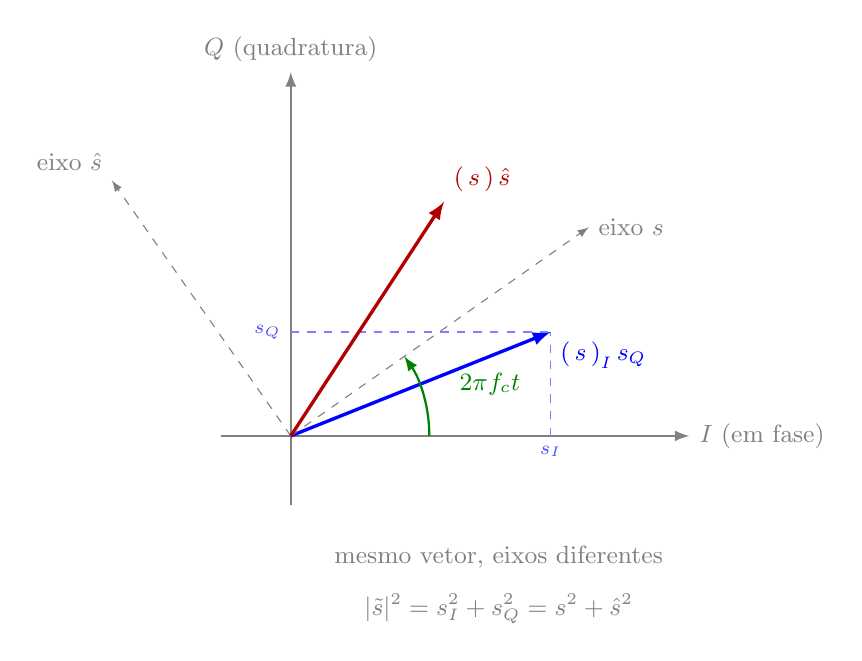
\begin{tikzpicture}[scale=2.2, >=latex]
% Original axes (I/Q)
\draw[->, thick, gray] (-0.4,0) -- (2.3,0) node[right, font=\small] {$I$ (em fase)};
\draw[->, thick, gray] (0,-0.4) -- (0,2.1) node[above, font=\small] {$Q$ (quadratura)};
% Original vector (baseband)
\draw[->, very thick, blue] (0,0) -- (1.5,0.6);
\node[blue, font=\small, below right] at (1.5,0.6) {$\begin{pmatrix}s_I \\ s_Q\end{pmatrix}$};
% Dashed projections for original
\draw[dashed, blue!50] (1.5,0) -- (1.5,0.6);
\draw[dashed, blue!50] (0,0.6) -- (1.5,0.6);
\node[blue!70, font=\scriptsize, below] at (1.5,0) {$s_I$};
\node[blue!70, font=\scriptsize, left] at (0,0.6) {$s_Q$};
% Rotated axes (s / s_hat)
\draw[->, gray, dashed] (0,0) -- ({2.1*cos(35)},{2.1*sin(35)}) node[right, font=\small] {eixo $s$};
\draw[->, gray, dashed] (0,0) -- ({-1.8*sin(35)},{1.8*cos(35)}) node[above left, font=\small] {eixo $\hat{s}$};
% Rotated vector
\pgfmathsetmacro{\rx}{1.5*cos(35)-0.6*sin(35)}
\pgfmathsetmacro{\ry}{1.5*sin(35)+0.6*cos(35)}
\draw[->, very thick, red!70!black] (0,0) -- (\rx,\ry);
\node[red!70!black, font=\small, above right] at (\rx,\ry) {$\begin{pmatrix}s \\ \hat{s}\end{pmatrix}$};
% Rotation arc
\draw[->, thick, green!50!black] (0.8,0) arc (0:35:0.8);
\node[green!50!black, font=\small] at (1.15,0.3) {$2\pi f_c t$};
% Same magnitude note
\node[font=\small, text=gray] at (1.2,-0.7) {mesmo vetor, eixos diferentes};
\node[font=\small, text=gray] at (1.2,-1.0) {$|\tilde{s}|^2 = s_I^2 + s_Q^2 = s^2 + \hat{s}^2$};
\end{tikzpicture}
\end{center}

\end{frame}

% ============================================

\begin{frame}{Modulador I/Q — Diagrama}

\begin{center}
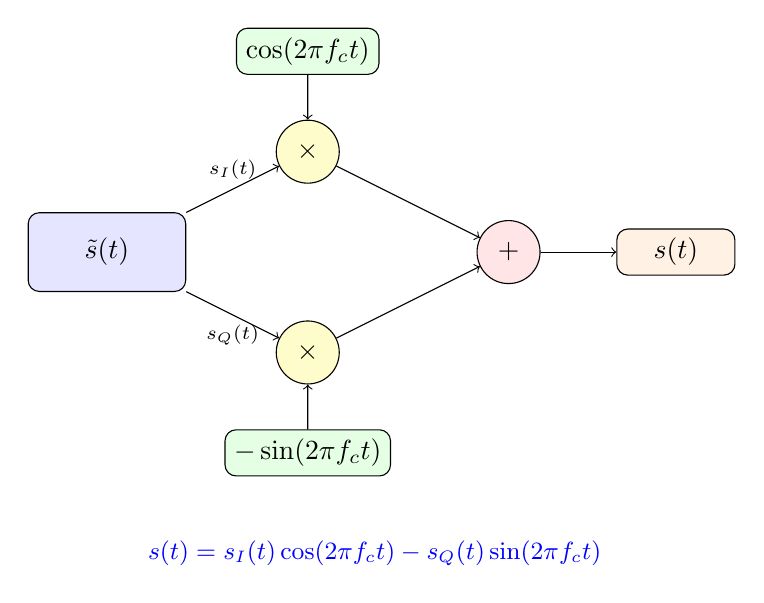
\begin{tikzpicture}[scale=0.85]
% Transmitter
\node[draw, rounded corners, fill=blue!10, minimum width=2cm, minimum height=1cm] (msg) at (0,0) {$\tilde{s}(t)$};
\node[draw, circle, fill=yellow!20, minimum size=0.8cm] (mix1) at (3,1.5) {$\times$};
\node[draw, circle, fill=yellow!20, minimum size=0.8cm] (mix2) at (3,-1.5) {$\times$};
\node[draw, rounded corners, fill=green!10] (cos) at (3,3) {$\cos(2\pi f_c t)$};
\node[draw, rounded corners, fill=green!10] (sin) at (3,-3) {$-\sin(2\pi f_c t)$};
\node[draw, circle, fill=red!10, minimum size=0.8cm] (sum) at (6,0) {$+$};
\node[draw, rounded corners, fill=orange!10, minimum width=1.5cm] (out) at (8.5,0) {$s(t)$};

% Connections
\draw[->] (msg) -- node[above,font=\scriptsize]{$s_I(t)$} (mix1);
\draw[->] (msg) -- node[below,font=\scriptsize]{$s_Q(t)$} (mix2);
\draw[->] (cos) -- (mix1);
\draw[->] (sin) -- (mix2);
\draw[->] (mix1) -- (sum);
\draw[->] (mix2) -- (sum);
\draw[->] (sum) -- (out);

% Label
\node[font=\small, text=blue] at (4,-4.5) {$s(t) = s_I(t)\cos(2\pi f_c t) - s_Q(t)\sin(2\pi f_c t)$};
\end{tikzpicture}
\end{center}

\textbf{Modulador I/Q:} Qualquer sinal passa-faixa pode ser representado por duas componentes de banda básica ($I$ e $Q$) modulando portadoras em quadratura.

\end{frame}

% ============================================

\begin{frame}{Envelope e Fase Instantânea}

Do sinal analítico $z(t) = s(t) + j\hat{s}(t)$, extraímos:

\vspace{-1mm}

\textbf{Envelope:} \quad $\boxed{a(t) = |z(t)| = \sqrt{s^2(t) + \hat{s}^2(t)}}$

\vspace{1mm}

\textbf{Fase instantânea:} \quad $\boxed{\theta(t) = \arg[z(t)] = \arctan\!\left(\frac{\hat{s}(t)}{s(t)}\right)}$

\vspace{1mm}

\textbf{Frequência instantânea:} \quad $\boxed{f_i(t) = \frac{1}{2\pi}\frac{d\theta(t)}{dt}}$

\vspace{2mm}

\textbf{Aplicação:} Detecção de envelope em AM, demodulação FM.

\end{frame}

% ============================================

\begin{frame}{Aplicação: Extração de Envelope em AM}

\begin{center}
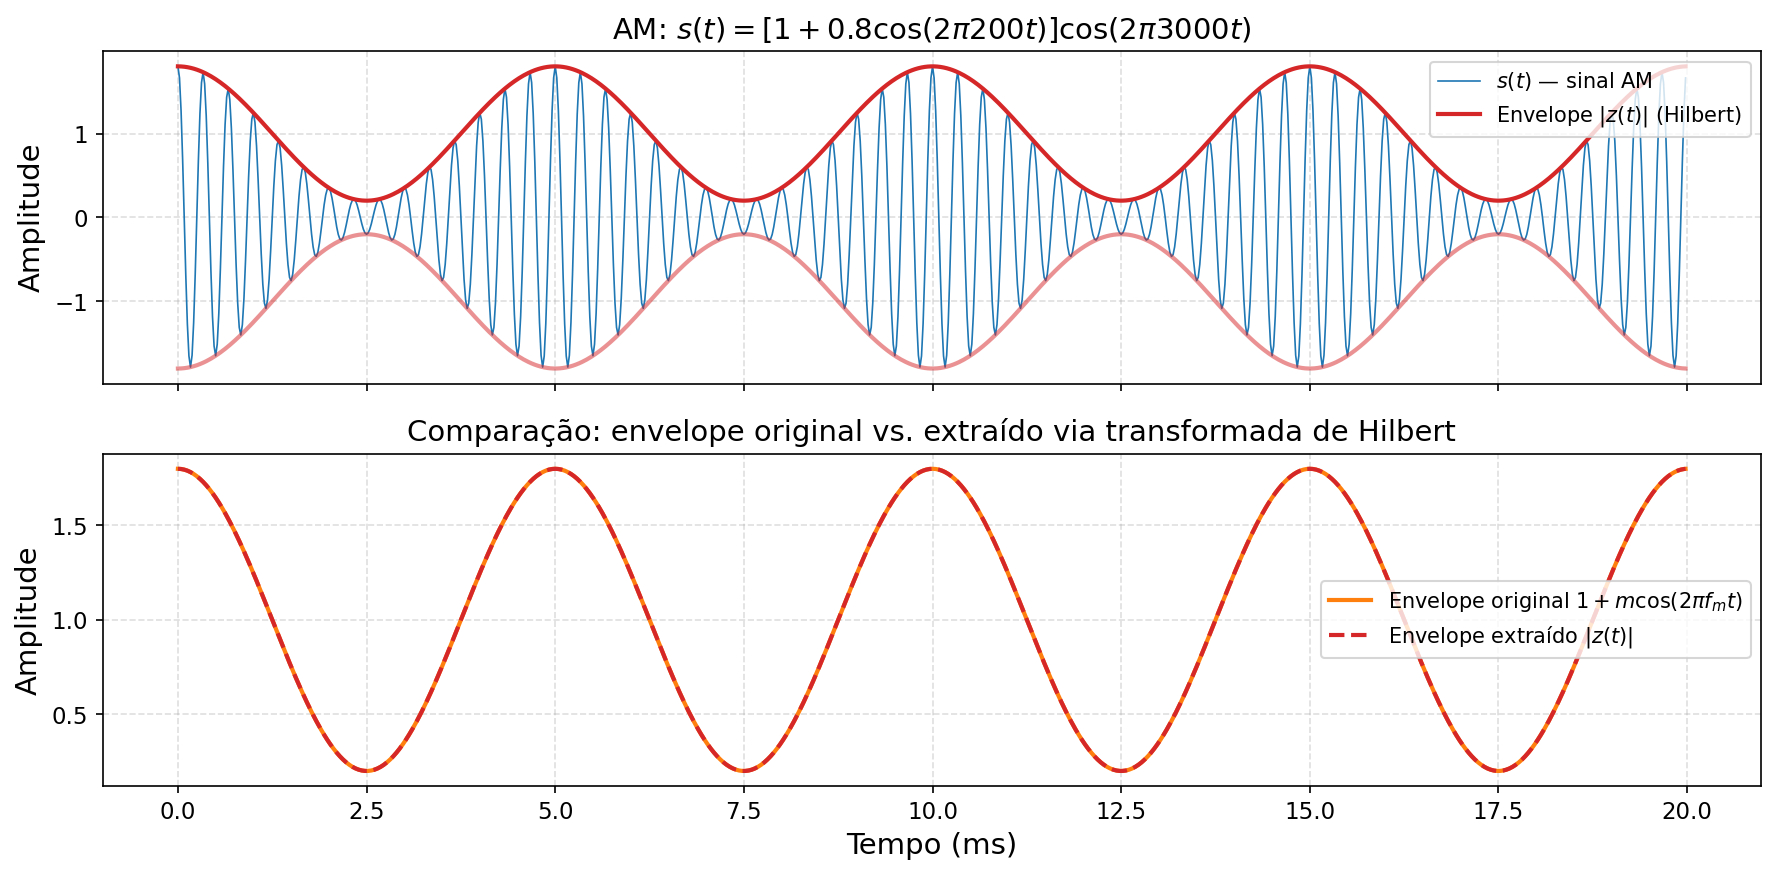
\includegraphics[width=\figFull, height=0.85\textheight, keepaspectratio]{figures/cap3/envelope_am}
\end{center}

\end{frame}

% ============================================

\begin{frame}{Resumo: Do Sinal Passante à Representação I/Q}

\begin{center}
\small
\begin{tabular}{|l|c|c|}
\hline
\textbf{Passo} & \textbf{Frequência} & \textbf{Tempo} \\
\hline
1. Sinal passante & $S(f)$ em $\pm f_c$ & $s(t)$ real \\
\hline
2. Sinal analítico & $Z(f) = 2S(f)\,u(f)$ & $z(t) = s(t) + j\hat{s}(t)$ \\
\hline
3. Envelope complexo & $\tilde{S}(f) = Z(f+f_c)$ & $\tilde{s}(t) = z(t)\,e^{-j2\pi f_c t}$ \\
\hline
4. Componentes I/Q & $\tilde{S}(f)$ em banda básica & $\tilde{s}(t) = s_I(t) + js_Q(t)$ \\
\hline
5. Reconstrução & $S(f)$ recuperado & $s(t) = s_I\cos - s_Q\sin$ \\
\hline
\end{tabular}
\end{center}

\vspace{0.3cm}

\textbf{Conexão fundamental:} A Transformada de Hilbert é a ponte entre sinais \textbf{reais} e \textbf{analíticos}, e entre representações de \textbf{banda passante} e \textbf{banda básica}.

\end{frame}


% ============================================
% SEÇÃO 3.10: COMPUTAÇÃO NUMÉRICA DA TRANSFORMADA DE FOURIER
% ============================================
\section{Computação Numérica: DFT e FFT}
\input{sec3_9_dft}
